\section{Introduction}

Reduced-order models (ROMs) enable repeated evaluation of high-fidelity dynamical systems at substantially reduced cost. Their construction becomes more difficult when parameter variation changes the qualitative dynamics of the system. Parameterized incompressible flows provide a representative example: different parts of the parameter domain may relax to a steady state, exhibit weak oscillatory growth near instability onset, or sustain nonlinear periodic motion. A useful ROM must therefore remain accurate under autonomous rollout across these regimes. After initialization from a short physical history, the model must evolve recursively using its own predictions, without access to future reference states.



This requirement exposes two coupled challenges. First, the reduced representation can be strongly regime dependent: a basis that efficiently represents nearly steady states may require substantially more degrees of freedom to represent developed periodic dynamics. Second, the reduced dynamics must describe qualitatively different temporal behavior, from relaxation toward a steady state to oscillatory growth and nonlinear periodic evolution. A global model must address both difficulties simultaneously, while autonomous rollout propagates prediction errors into subsequent states. The challenge is therefore not simply one of model capacity: a single global reduced space may require additional dimensions to accommodate regime-specific structures, while a single dynamical model must approximate qualitatively different behaviors within one parameterization.


Projection-based ROMs provide an explicit reduced representation and reduced dynamics, commonly through proper orthogonal decomposition (POD) and
Galerkin projection \citep{sirovich1987,berkooz1993,benner2015}. Truncation, however, removes interactions that can still influence the retained coordinates, producing closure errors that degrade long-horizon prediction \citep{amsallem2012}. Data-driven reduced models offer greater flexibility in approximating nonlinear dynamics, but low one-step error does not guarantee accurate autonomous rollout \citep{pathak2018,vlachas2018,duraisamy2019,brunton2020}. Hybrid ROMs combine physics-based reduced models with learned corrections or learned reduced representations, retaining physical structure while increasing approximation flexibility
\citep{dar2023,lee2020,fresca2022,geelen2023}. A complementary strategy localizes the reduced representation, using multiple subspaces, clusters, or manifolds for different portions of the solution set \citep{kaiser2014,li2021cluster,diaz2024}. These directions address complementary aspects of the broad-parameter problem: hybrid modeling improves the fidelity of the reduced dynamics, whereas localization adapts the reduced representation to regime-dependent structure.

Localization, however, creates a new assembly problem. Independently constructed local ROMs generally have different mean fields, bases, scalings, and reduced operators, so their coefficient vectors are not componentwise comparable. Direct interpolation or averaging in reduced-coordinate space therefore has no natural cross-chart interpretation. Mixture-of-experts (MoE) architectures provide a natural framework for conditional specialization \citep{jacobs1991,jordan1994,shazeer2017,fedus2022}, but many standard MoE formulations route specialized predictors within a shared representation or common feature space. The resulting problem is therefore hierarchical: one must adapt the reduced dynamics within each local representation and, separately, select or combine complete local ROMs across representations that do not share coordinates. This raises a distinct question that standard within-representation MoE routing does not address: how can independently constructed local dynamical models be assembled without forcing them into a common latent coordinate system?


To address this gap, we introduce the Regime-Adaptive Localized Mixture-of-Experts Reduced-Order Model (RAL-MoE-ROM), a two-level hierarchy that separates within-regime dynamical specialization from cross-regime model selection and assembly. The parameter domain is covered by overlapping regime-local parameter regions, each equipped with an independent reduced chart and a complete autonomous specialist. Within each specialist, the projected ROM backbone is augmented by a structured sparse MoE correction for unresolved reduced dynamics. Each specialist undergoes closed-loop rollout training, so that its learned correction is optimized under the recursive inputs encountered at inference. At the second level, an outer parameter-only regime router (E2) assigns a trajectory-level preference over local specialists. When two adjacent specialists are both applicable, a learned Top-2 convex fusion (T2-C) uses recent physical history to refine their relative weight. The selected specialists encode the same physical history in their own coordinates and evolve independently. Their predictions are combined only after reconstruction in the common physical space, and the fused output is not fed back into either local trajectory.


Our contributions are threefold:
\begin{itemize}
    \item \textbf{A two-level hierarchical MoE for reduced dynamics.}
    The first level performs sparse conditional correction within each
    regime-local ROM, while the second selects or combines complete local
    ROMs across regimes. This separates within-regime dynamical
    specialization from cross-regime model selection.

    \item \textbf{Structured autonomous regime-local specialists.}
    Each specialist retains an explicit projected ROM backbone and augments
    it with sparsely routed structured corrections trained under closed-loop
    rollout. The correction experts combine nonlinear, linear, and low-rank
    quadratic responses, providing flexible unresolved dynamics without
    replacing the underlying projected model.

    \item \textbf{Physical-space assembly across independent local ROMs.}
    Adjacent specialists retain independent coordinates and autonomous
    trajectories. T2-C combines only their reconstructed physical fields
    through a history-conditioned convex weight, avoiding direct
    interpolation of reduced states or operators.
\end{itemize}

\par
\begin{figure}[t]
    \centering
    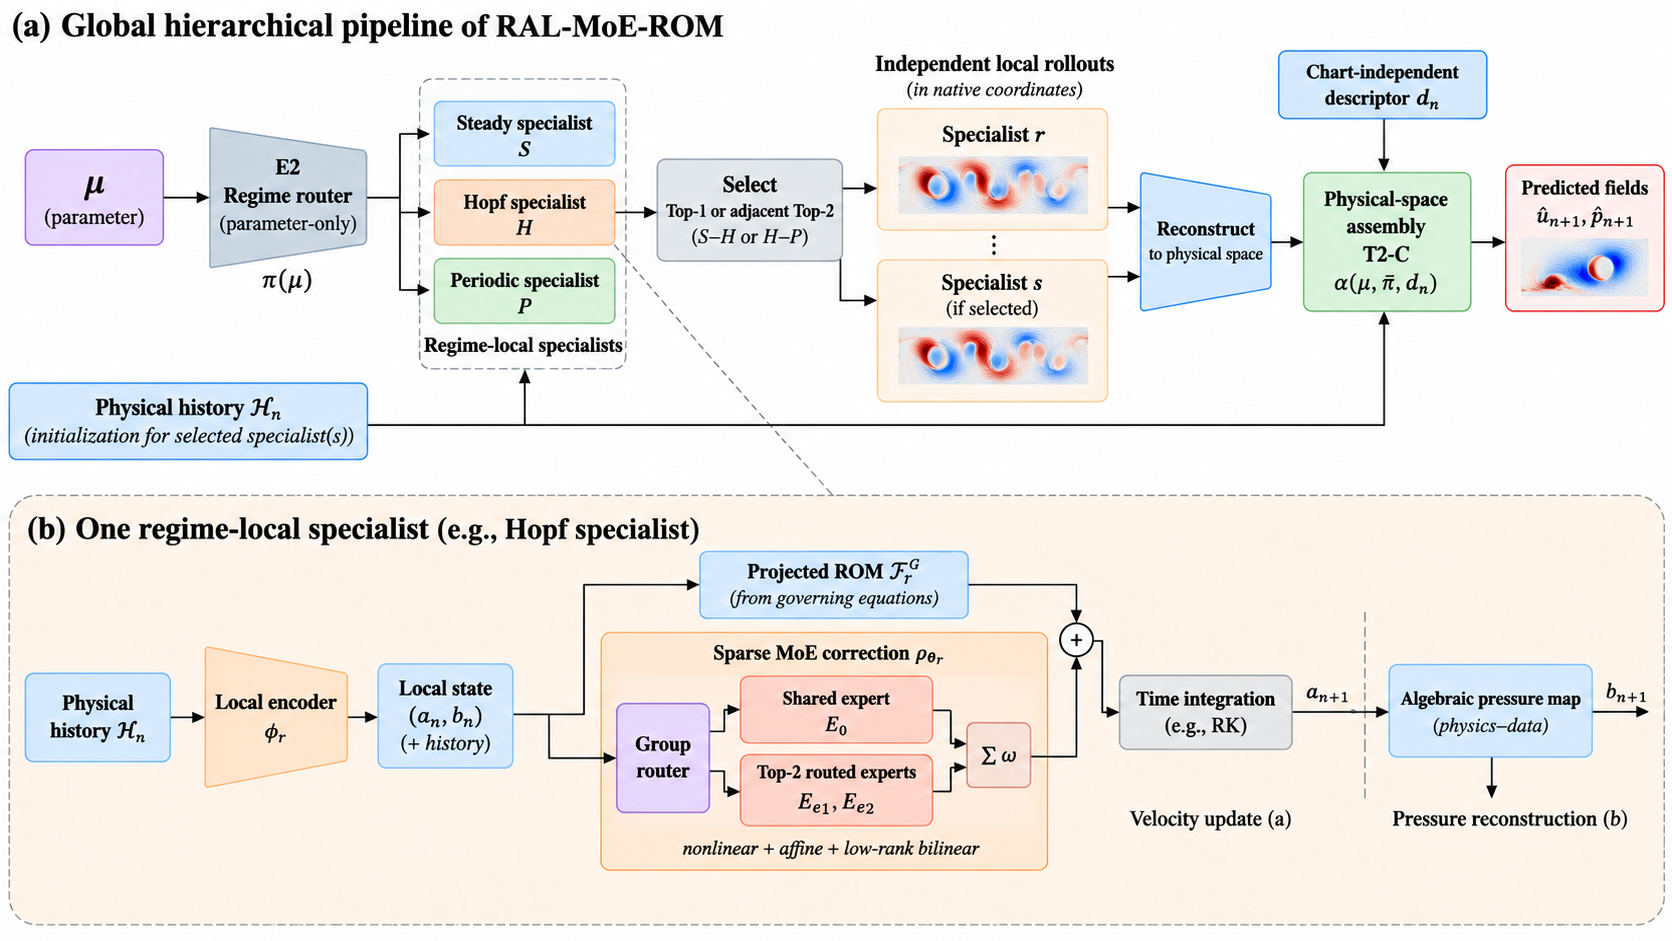
\includegraphics[width=\linewidth]{figures/ral_moe_rom_overview_user_20260908.png}
    \caption{
    Overview of RAL-MoE-ROM.
    (a) A parameter-only outer router selects one regime-local specialist or an adjacent pair. Selected specialists encode the same physical history in their native coordinates, evolve independently, and are combined only after reconstruction; recent physical history conditions the Top-2 fusion but not the outer router. (b) Each specialist augments the projected Galerkin backbone with a structured sparse MoE correction, while pressure is reconstructed algebraically. Flow thumbnails are schematic.
}
    \label{fig:ral_overview}
\end{figure}
\par
